\documentclass[12pt]{article}

\textwidth 16.5cm
\textheight 22.5cm
\oddsidemargin 0pt
\topmargin -1cm
\parskip 0.3cm

\RequirePackage[colorlinks,citecolor=blue,urlcolor=blue,breaklinks]{hyperref}
\usepackage{psfrag}
\usepackage{graphicx}
\usepackage{graphics}
\usepackage{latexsym,amsmath,amssymb,amsfonts,amsthm,bbm,enumerate, color}
\usepackage{natbib}
\usepackage{xr}

\usepackage{xcolor}
\usepackage[draft,inline,nomargin,index]{fixme}
\fxsetup{theme=color,mode=multiuser}
\FXRegisterAuthor{tc}{atc}{\color{red} TC}
\FXRegisterAuthor{jb}{ajb}{\color{red} JB}

\newcommand{\qu}[1]{`#1'}
\newcommand{\hyp}[2][]{#1~\ref{#2}}
\newcommand{\hype}[1]{\eqref{#1}}


\renewcommand{\thefootnote}{\fnsymbol{footnote}}

\newcommand{\red}[1]{\textcolor{red}{#1}}
\newcommand{\blue}[1]{\textcolor{blue}{#1}}
\newcommand{\green}[1]{\textcolor{green!60!black}{#1}}
\newcommand{\orange}[1]{\textcolor{orange!90!black}{#1}}

\newcommand{\vtwo}[1]{\textcolor{red}{#1}}


\newcommand{\vertiii}[1]{{\left\vert\kern-0.25ex\left\vert\kern-0.25ex\left\vert #1 
    \right\vert\kern-0.25ex\right\vert\kern-0.25ex\right\vert}}
\newenvironment{prooftitle}[1]{{\noindent \textsc{Proof #1}}\\}


\begin{document}

\begin{center}
\Large{\textbf{Response to the reviewers}}
\end{center}

\vspace{0.2in}

{\large \textbf{Reply to the Editor}}

Dear Ananya,

Thank you very much for your decision on our manuscript on the 6th July.

\textbf{Your manuscript ``Data-driven design of targeted gene panels for estimating immunotherapy biomarkers" has now been seen by 3 referees, whose comments are appended below. You will see that while they find your work of interest, they have raised points that need to be addressed before we can make a decision on publication. }

We are very grateful to you and the three reviewers for their helpful and constructive comments, and we have revised the paper accordingly.  The main changes are as follows: 
\begin{itemize}
    \item We have \tcnote{Section 3.3} ... 
    \item \tcnote{We have included a new Section 4 which covers several further analyses on different cancer types. } 
    \item \tcnote{We include in our conclusion section a detailed discussion of the potential limitations of our method -- see also our detailed response to referee 3.} 
\end{itemize}
Please also see our detailed point-by-point response to the reviewers comments below.  All changes in the main text are highlighted in \vtwo{red}.

%\textbf{The referees’ reports seem to be quite clear. Naturally, we will need you to address all of the points raised. } \textbf{While we ask you to address all of the points raised, the following points need to be substantially worked on:} \textbf{- Please provide all details of the method and the model as pointed out by reviewer~1.}\textbf{- Please verify the generalization of the proposed method as requested by reviewer~1.}\textbf{- Reviewer~2 has mentioned that the general utility of the model needs to be explored.}\textbf{- Reviewer~3 has pointed out the need for validation of the method on datasets in which response to immunotherapy is available.}\textbf{- Please show how robust the classifier is to different TMB thresholds.}\textbf{- Please compare the methods with other panel selection methods such as the ones mentioned in the introduction section as requested by Reviewer~1.}\textbf{- Please discuss the underlying flaws in the study as pointed out by Reviewer 3.}

Thank you in advance for your continued handling of our paper.  We look forward to hearing from you soon. 

Best wishes,

Tim (also on behalf of Jacob)

\bigskip 


\clearpage


{\large \textbf{Reply to Referee 1}}

\textbf{In this paper, Bradley and Cannings developed a generative model for the design of target gene panel to estimate the immunotherapy biomarker, tumor mutation burden (TMB). The topic is important since identification of potential predictive biomarkers is critical to optimize the benefits of immunotherapy in patients. The performance of the developed method seemed to be good. However, some concerns need to be clarified before publication.} 

Thank you for this summary and your helpful feedback below.

\textbf{1. Some details about the method and the model are missing. 
(a) In line 132, why do you use log-link function to model the dependence of the mutation rate on the sample, gene and mutation type? Specifically, why does gene length need log and others do not?
(b) In line 149, what is the biological meaning of mutation rate – mutation * log(mutation rate)?
(c) In line 147, what if all parameters are penalized?
(d) In line 366, why does the selection procedure tend to favor genes with higher overall mutation rates?}

Thank you for these questions.  To clarify (a), the log link function is the canonical link function used in Poisson regression. It means that a linear change in any of the parameters in equation (3), results in a multiplicative change in the mutation rate (this also ensures that mutation rate is positive).  As mentioned in the paper,  we use to offset $\log(\ell_g)$ to model that the mutation rate is proportional to the length of a gene (ie. $\phi_{igs} \propto \ell_g$). The other parameters are not taken on the log scale, so that if a parameter is not contributing to the mutation rate then its value will be exactly 0.  
For your second point, this term arises in the negative log-likelihood; it can be interpreted as a measure of how well the observed mutation count agrees with our Poisson model. It shouldn't be interpreted to have any direct biological meaning. 

Regarding (c), penalising the parameter $\nu_s$ would correspond to the belief that different mutation types occur at the same rate, and similarly, penalising $\mu_i$ would correspond to many tumours having the same BMR. We typically don't think that this would be the case, but the penalty may be included if desired. To add more detail, in our revision we now write:
\begin{quotation}
    We do not penalise the parameters $\nu_s$ or $\mu_i$ since we expect that different mutation types occur at different rates, and that the BMR is different in each sample.
\end{quotation}

For your last question, our selection procedure favors genes with higher mutation rates since the signal to noise ratio for these genes is higher.  To see this, suppose that $X_1 \sim \mathrm{Poisson}(\alpha_1 t)$ and $X_2 \sim \mathrm{Poisson}(\alpha_2 t)$ are independent random variables with known relative mutation rates $\alpha_1,\alpha_2 > 0$. Then the maximum likelihood estimate of $t$ is $\hat{t} = \frac{X_1 + X_2}{\alpha_1 + \alpha_2}$, and we have that $\mathbb{E}(\hat{t}) = t$ and $\mathrm{Var}(\hat{t}) = \frac{t}{\alpha_1+\alpha_2}$, therefore the variable (either $X_1$ or $X_2$) with the larger relative mutation rate provides more information about $t$ (in terms of mean squared error). In fact, if either $\alpha_1$ or $\alpha_2$ are very small, then it may be preferable to estimate $t$ using just the variable with the larger mutation rate and not incur the cost of measuring the other variable.   %In other words, the genes with high mutation rates are more reliable predictors of the overall number of mutations.

We have opted against including these extra details in our revision, but we will incorporate them if you feel strongly.  Nevertheless we have modified the original sentence in our revision to better clarify the effect that selecting highly mutated genes has on the count estimator.  We now write
\begin{quotation}
This is because our selection procedure tends to favour genes with higher overall mutation rates and thus a count estimator based on the highly mutated genes will overestimate the  total number of mutations.
\end{quotation}



\textbf{2. Based on the developed framework, the authors applied the methods on a set of NSCLC data and evaluate the performances. The results shown in the manuscript indicate that their approach outperforms others. However, in my opinion, the authors should verify the generalization of the proposed method. First, the authors need to apply the proposed methods in other cancer types and evaluate the performance. Second, the authors need to use data from other studies for performance evaluation. For example, the authors train the model using the NSCLC data from \citet{campbell_distinct_2016} and then test the performance in other datasets such as data from TCGA. Third, in addition to the commonly used gene panels and ecTMB, the authors need to compare their methods with other panel selection methods such as the one mentioned in the introduction section.}

\tcnote{This will be covered in our main changes -- i.e. evaluating the performance on different data. }  

Thank you also for your third suggestion. We have now included the comparison on the panel selected by the proposal of \citet{lyu_mutation_2018} in Figure~7 of our revision. 

\textbf{3. In line 272, the authors indicated they randomly split the dataset into training, validation and test sets, which contain $n_{train} = 800$, $n_{val} = 171$ and $n_{test} = 173$ samples. I think the authors should perform the random split multiple times to verify the robustness of the proposed method.}

Thank you for this suggestion. A key aspect of our analysis, and in particular the split into disjoint training, validation and test sets, is that the test set has only been used once to evaluate performance for each prediction task (that is in Figure~8 for estimating TMB, Figure~10 for TIB and Table~2 for panel augmentation). This ensures that we have unbiased estimates of the true predictive performance in each case; crucially we have no selection bias or overfitting to the test set. Moreover, the separate training and validation sets are used to ensure again that there is no selection bias when we choose the appropriate panel size. Using many different random splits may result in overfitting and optimistic reporting of the results.  

Nevertheless, robustness is of course a key consideration -- we hope that the additional analysis we have now included in response to your Point 2 using different datasets demonstrates the our method is indeed robust. \tcnote{revisit this after responding to point 2}

\textbf{4. In line 135, parameter $\mu_i$ corresponds to the background mutation rate. I wonder that is there significant correlation between the identified $\mu_i$ and the status of cigarette smoking for the sample? In other words, does higher $\mu_i$ indicate more cigarette smoking? This should be clarified since the authors claimed that their work has the scope to help understand mutational processes in the conclusions section.}

This is an interesting question.  We have calculated the association between $\mu_i$ and smoking status in our training dataset. Non-smokers had an average BMR (with standard deviation in brackets) of 4.04 (1.12), reformed smokers 5.26 (0.84) and current smokers 5.40 (0.76). Indeed, as expected those with higher $\mu_i$ are more likely to be smokers.  We have opted against including this in the manuscript since we have not designed the study to investigate such an association. In order to clarify the scope of the discussion in Section 5 (previously Section 4), we now write at the end of the penultimate paragraph:
\begin{quotation}
Of course, any such associations need to be carefully investigated in follow up studies.
\end{quotation}

\textbf{5. Some contents are not consistent across the manuscript.
(a) The NSCLC data for analysis is from \citet{campbell_distinct_2016}, not from \citet{chalmers_analysis_2017} (line 61 and line 98).
(b) The panel used for panel augmentation case study should be TST-170 panel (line 408) rather than FoundationOne (line 266).}

Thank you for pointing out these typos, they have been corrected in our revision. 

\textbf{6. Some minor things to be confirmed:
(a) In line 140: should the free parameters be $n + |G| + |S| + |G||S|$?
(b) In Figure 4, it seems that only 4 largest negative genes are labeled.}

Thank you for these points. (a) The number of free parameters is given as follows: there a $n$ parameters $\mu_i$ for $i = 1, \ldots, n$, $|G|$ parameters $\lambda_g$ for $g \in G$, $|S|$ parameters $\nu_s$ for $s \in S$, and $(|S| - 1) |G|$ parameters $\eta_{gs}$ for $g \in G$ and $s \in S \setminus \{s_1\}$. Note in particular (as mentioned in line 134) that $\eta_{gs_1} = 0$ for all $g \in G$, thus these last $|G|$ parameters are fixed to be zero and do not contribute to the total number of free parameters. In total we do therefore have $n + |G| + |S| + (|S|-1)|G| = n + |S| + |S||G|$ free parameters as stated in the paper.  We hope that clarifies things; we will happily add these extra details to the paper if needed. (b) In figure 4, we have only labelled the 5 largest gene parameters (and none of the negative gene parameters), unfortunately the previous formatting of the figure meant that the labels overlapped -- this has been rectified in our revision. 

\textbf{7. The format of the references need modification. Specifically, the papers with more than three authors only showed the first three authors in the references.}

Thank you -- the references are now correctly formatted. 


\begin{thebibliography}{75}
\bibitem[Campbell et al.(2016)]{campbell_distinct_2016} Campbell, Joshua D. and Alexandrov, Anton and Kim, Jaegil and Wala, Jeremiah and Berger, Alice H. and Pedamallu, Chandra Sekhar and Shukla, Sachet A. and Guo, Guangwu and Brooks, Angela N. and Murray, Bradley A. and Imielinski, Marcin and Hu, Xin and Ling, Shiyun and Akbani, Rehan and Rosenberg, Mara and Cibulskis, Carrie and Ramachandran, Aruna and Collisson, Eric A. and Kwiatkowski, David J. and Lawrence, Michael S. and Weinstein, John N. and Verhaak, Roel G. W. and Wu, Catherine J. and Hammerman, Peter S. and Cherniack, Andrew D. and Getz, Gad and {Cancer Genome Atlas Research Network} and Artyomov, Maxim N. and Schreiber, Robert and Govindan, Ramaswamy and Meyerson, Matthew (2016) Distinct patterns of somatic genome alterations in lung adenocarcinomas and squamous cell carcinomas, \emph{Nature Genetics}, \textbf{48}, 607--616.

\bibitem[Chalmers et al. (2017)]{chalmers_analysis_2017} Chalmers, Z. R., Connelly, C. F. and Fabrizio, D. (2017) Analysis of 100,000 human cancer genomes reveals the landscape of tumor mutational burden, \emph{Genome Medicine}, \textbf{9}, 34.

\bibitem[Lyu et al.(2018)]{lyu_mutation_2018} Lyu, G.-Y., Yeh, Y.-H. and Yeh, Y.-C. (2018) Mutation load estimation model as a predictor of the response to cancer immunotherapy. \emph{Nature Genomic Medicine}, \textbf{3}, 1-9.
\end{thebibliography}

\clearpage

{\large \textbf{Reply to Referee 2}}

\textbf{In their manuscript entitled ‘Data-driven design of targeted gene panels for estimating immunotherapy biomarkers’, Drs Bradley and Cannings introduce a new model for inferring tumor mutational burden from targeted NGS panels. Their model is biologically relevant, insofar as it considers sample and gene specific mutation rates, and they demonstrate good performance of the model in predicting sample TMB classification. While their model allows for design of a targeted panel that more accurately infers TMB, they demonstrate that their TMB estimation from a pre-specific gene list performs as well or better than other TMB estimation approaches.}

Thank you for summarising our work, and for your constructive comments below. 

\textbf{1. Ultimately the biggest concern is about the practical utility of this model. The authors demonstrate good performance with the sample set, but would benefit from demonstrating that this approach performs well in tumor types with lower mutation rates and less prominent mutational processes, such as renal cell carcinoma, breast, and prostate cancer.}

\tcnote{This will be done in our main revision}

\textbf{2. Additionally, the NSCLC cohort used in this analysis includes both squamous and non-squamous NSCLC. Does the model perform equally well on both? What about in tumors without dominant smoking signature (e.g. EGFR mutated samples or from never smokers)? What about microsatellite stable vs unstable colorectal cancer? These subgroup analyses would help clarify how precise the training and validation datasets need to be relative to the underlying mutational process. }


These are interesting questions.  For your first point, the performance in the test set for squamous cells was $R^2 = 0.77$ and for non-squamous cells was $R^2 = 0.91$. Further, the regression performance on EGFR mutated samples was $R^2 = 0.92$ and for never smokers was $R^2 = 0.84$.  However, we need to be extremely careful in performing these kind of subgroup analyses (especially with small sample sizes), and since our study was not designed to investigate any particular subgroups, we have decided not to report these subgroup specific results in the paper.  Similarly for your final point, which is of course of interest, one would need to carry out a carefully designed follow-up study in order to conclusively report valid subgroup analyses, which is beyond the scope of this work.  

\textbf{3. Discrepancies between WES and panel-derived TMB arise not only from gene downsampling, but also from differences in the performance of sequencing assays (sample processing, sequence coverage, artifacts, etc).}

Thank you for this comment. Technical variation is indeed another key consideration for the accuracy of gene panel-based sequencing. We hope that our inclusion of external test data (see the new Sections 3.3 and 4) demonstrates robustness to study effects.   

\textbf{4. Similarly, the authors apply their model to a specific TMB cut-off; many previously selected TMB cut-offs are around the 50th percentile; how robust is the classifier to different TMB thresholds?}

Thank you for this question.  The main aim of our proposal is to predict TMB directly via a regression model, and our model does not depend on the classification step (in particular it doesn't depend on the cutoff of 300 mutations used in Section 3;  note that 300 corresponds to around 10 mutations per megabase, and to around the 75th percentile of TMB values).  In fact, the classification performance for different TMB cutoffs may be informally assessed by further inspection of the plot in top left panel of Figure~8.  For example the recall is the number of points in the top right quadrant divided by the number of points in the top two quadrants.  This calculation may be carried out for any TMB cutoffs by moving the appropriate horizontal and vertical grey dotted lines. 

We calculated the classification performance on the NSCLC dataset for different high/low TMB thresholds -- see the figure below.   We see that the classifier is indeed robust to the different thresholds; the area under the receiver operating characteristics curves (AUROC) and the precision recall curves (AUPRC) are all above 0.93 (an AUROC or AUPRC of 1 corresponds to perfect classification).  %Note that while classification typically becomes harder in terms of precision and recall as the TMB cutoff quantile increases (this is due to the fact that minority class is smaller and cases in that class are harder to identify), the performance of our classifier remains high since it is based on thresholding a regression estimate.  

\begin{figure}[htbp]
\centering
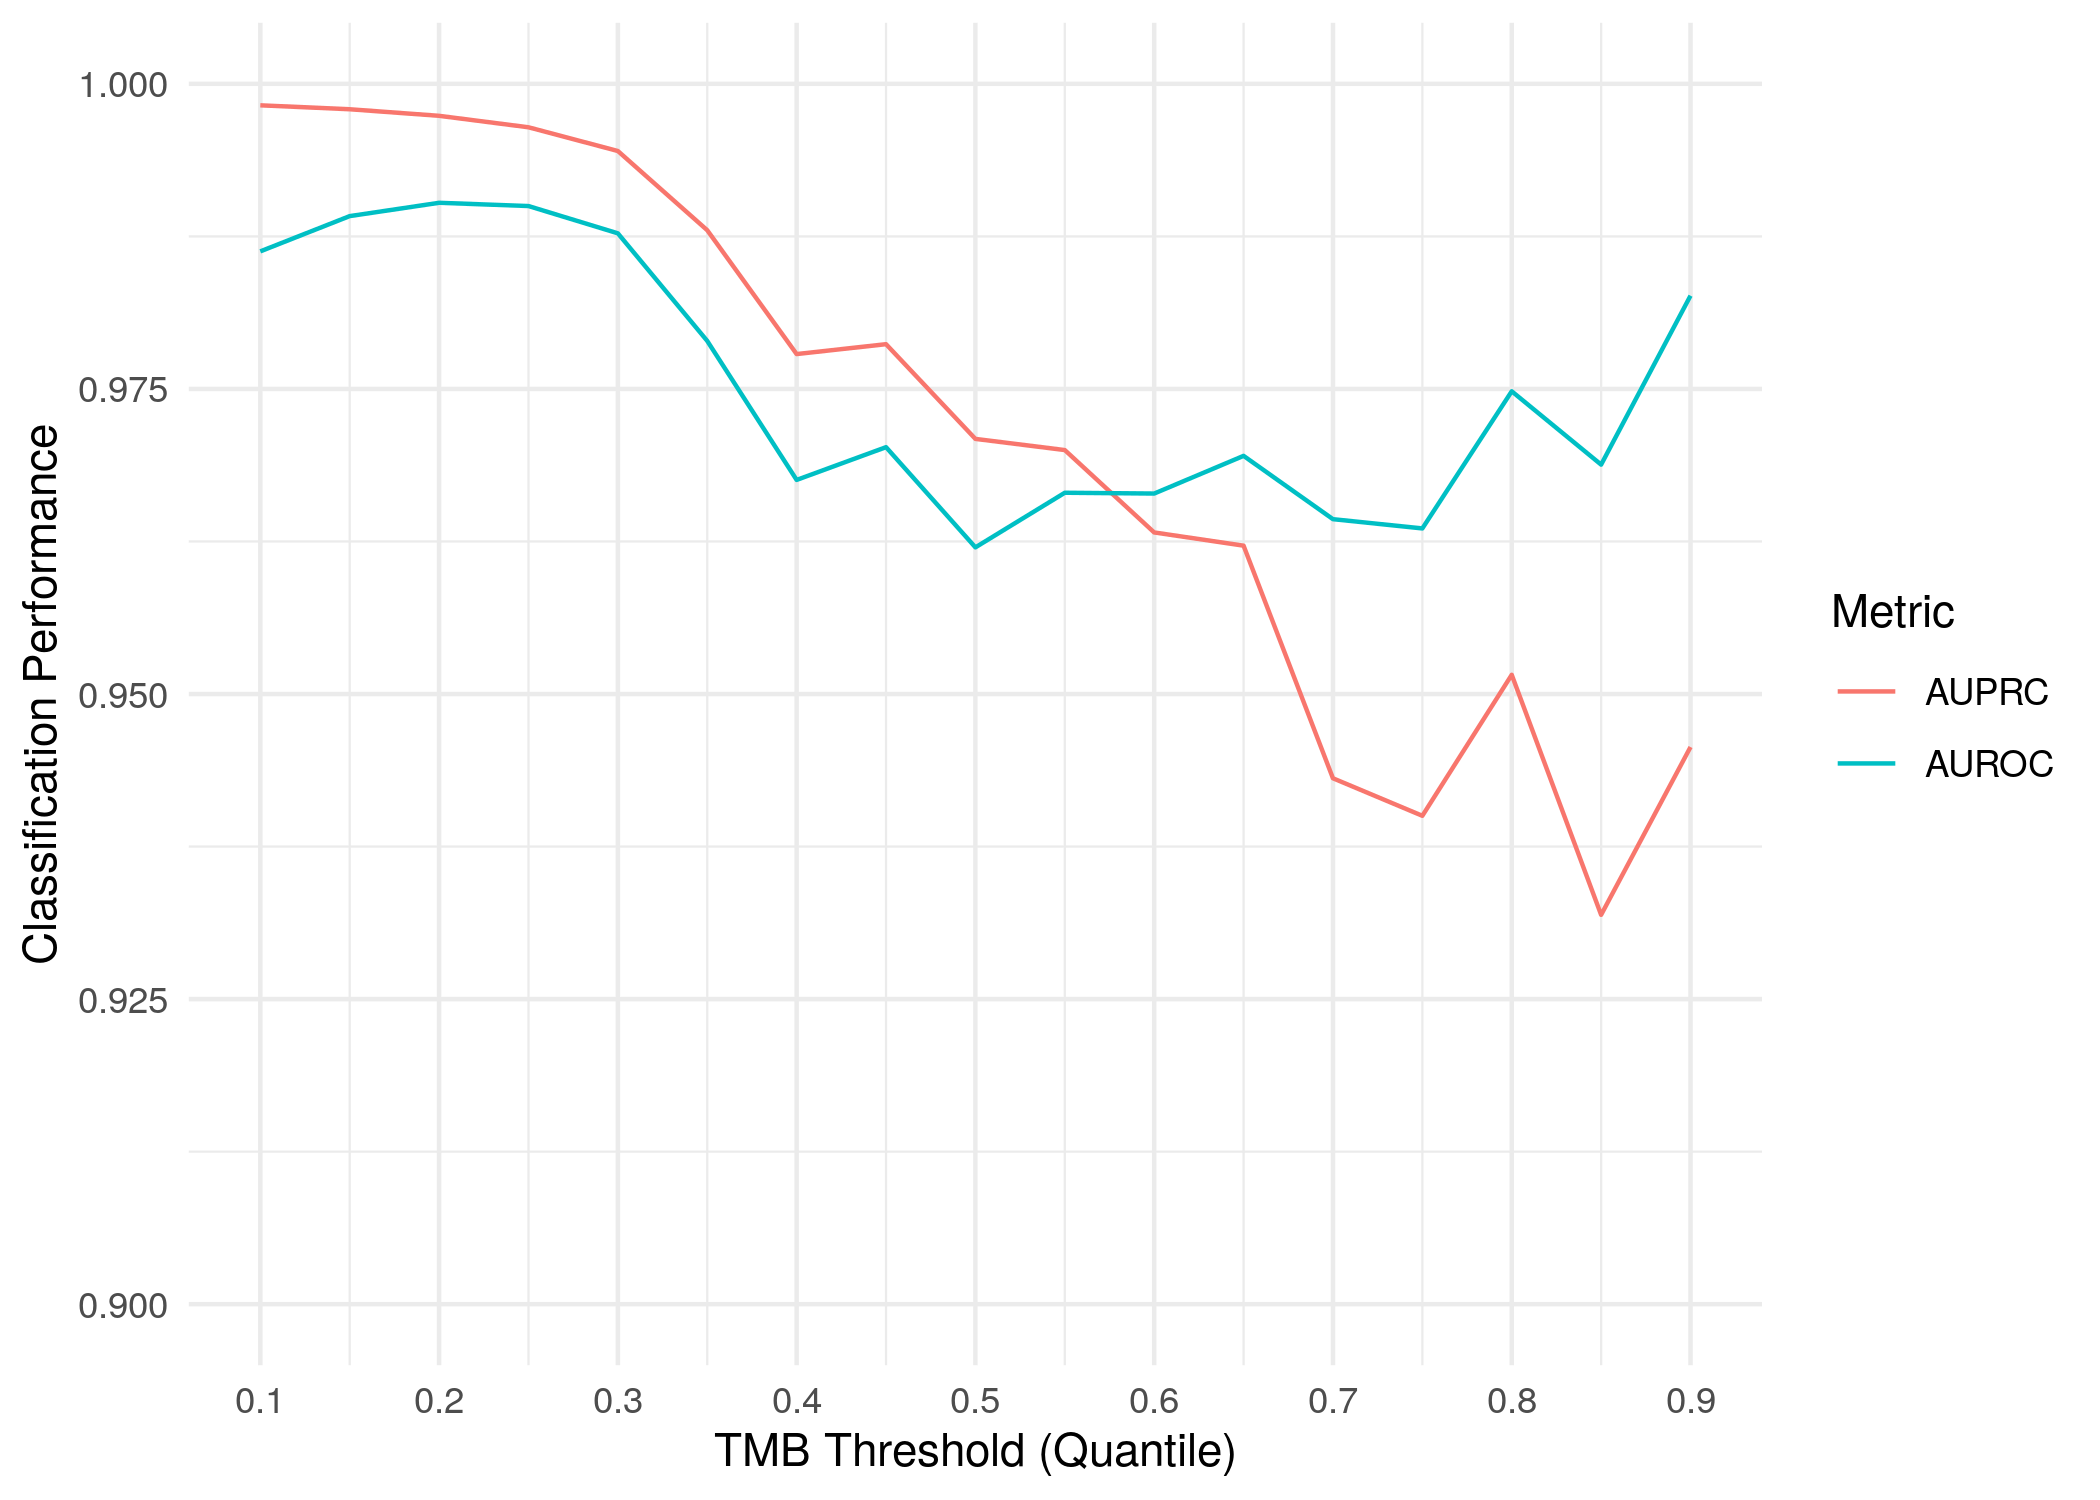
\includegraphics[width=4in]{../../results/figures/quantile_thresholds_fig.png}
%\caption{}
\end{figure} 

We feel that, since the reader can get an intuitive sense of the model's robustness in terms of classification performance from Figure 8, the extra detail here adds little to what we have presented in the paper, and have opted against including these additional calculations.  We will of course reconsider and include this if you feel strongly.  

\textbf{Minor points: 1. KRAS is an oncogene, not a tumor suppressor gene}

Thanks -- we have corrected this in our revision. 

\begin{thebibliography}{75}

\end{thebibliography}

\clearpage

{\large \textbf{Reply to Referee 3}}

\textbf{The authors propose an algorithm to optimise the design of targeted sequencing panels for the correct quantification of Tumor Mutational Burden (TMB). The issue is at the center of debated discussion in the immune-oncology community, since histology-agnostic treatments have been approved by the FDA for treating tumors purely on the basis of an elevated TMB quantified by a specific commercial platform and a specific cutoff; thus, the possibility to obtain TMB quantification using alternative platforms is highly sought after, given the increasing diffusion of genome sequencing in clinical routine. Adequate TMB estimation through targeted panels has been hampered by the need to keep the sequencing space low in order to maintain financial sustainability and to enrich for clinically actionable genomic regions. The authors’ work operates within this landscape and proposes an algorithm that helps practitioners to design custom panels with optimal TMB estimation. They attempt to
validate their results on public cancer sequencing datasets and simulate their performance starting from sequencing panels in use.}

Thank you for your detailed discussion of our work.  

\textbf{Although the question asked and the methodology used are of interest, there are some fundamental flaws with the underlying logic of the study that undermines its actual utility in 2021. The final purpose of any TMB quantification is to identify patients at high likelihood of responding to immune checkpoint inhibitors, with the underlying assumption that high TMB is a good proxy for neoantigens, and the further assumption that high neoantigen load drives high responses. Since none of these are actual equivalences but only partial correlations, it is not surprising that several recent analyses (e.g.~\citet{litchfield2021meta}) highlighted that TMB alone is a poor predictor of immunotherapy response: additional factors, themselves partially co-varying with TMB (and thus confounding) play a role and cannot be left out: without considering gene expression-based phenotypes, these factors include mutation type (partially addressed in the paper, through the separate discussion on indel
burden), identity of the mutated genes, aneuploidy and, most importantly, tumor histology.}

Thank you for these points, we're glad to hear that you found our proposed methodology interesting.  The main goal of our work is to develop a framework for the data-driven selection of gene panels which then allow for accurate prediction of exome-wide biomarkers such as TMB and TIB.  As you point out the main use of TMB is to identify patients that are more likely to respond to immunotherapy (indeed in \citet{litchfield2021meta} TMB was found to be among the best single predictors of checkpoint immunotherapy response, TIB was also identified as a significant single predictor).  Of course, if the goal is to predict response to immunotherapy, then one would attempt to identify a number of factors that may be used to train a classifier; as you suggest these may include cancer type (including subtype),  the presence of mutations in particular genes, aneuploidy and tumor histology. One would also consider a range of other variables, such as gender, age and exogenous factors. Nevertheless, one would certainly like to include TMB as a factor in any classifier, both due to its widely acknowledged use as a predictive biomarker and its clear interpretation from a clinical perspective.  It is very appealing therefore to obtain accurate and cost effective estimators of TMB (and other biomarkers such as TIB).  

The main goal of this work is to predict exome-wide biomakers using a data-driven gene panels, we have therefore opted against fully developing a classifier of response to immunotherapy as we feel this is outside the scope of our work.  Nevertheless we now demonstrate that our predictions of TMB may be used in place of the true TMB when classifying response to immunotherapy -- see the new Section 3.3 and our response to your third point below. 

We now also discuss the utility of our predictions of TMB and TIB in Section 5, where we now write:
\begin{quotation}
The main use of TMB is often to help identify patients that are more likely to respond to immunotherapy. While TMB is a good single predictor of response \citep{cao_high_2019, zhu_association_2019}, it is of course desirable to improve the predictive performance by including other factors, these may include  cancer type (and subtype), specific mutational signatures, aneuploidy and tumor histology, as well as other variables, such as gender, age and exogenous factors. Indeed, \citet{litchfield2021meta} show that, by including markers of T-cell infiltration and other factors, a multivariate predictor of response to immunotherapy significantly improves the classification performance in comparison to using TMB alone.  Nevertheless, one would certainly like to include TMB (or a closely related measure) as a factor in any classifier of response.
\end{quotation}


\textbf{This is a particularly weak point for the study, since the validations are only conducted on NSCLC genomes coming from early studies, which have mutational landscapes that are intrinsically different from other tumor types in which TMB identification is clinically relevant (e.g. melanoma, urothelial); in other words, the model may be overfit for the NSCLC landscape, while it purports to be applied across all histologies (if it was not histology-agnostic and admittedly restricted to NSCLC, it would fail its scope, since TMB as a criterium for immunotherapy prescription is FDA approved in histology-agnostic fashion).}


\tcnote{I think we will be able to give a strong response to this after we have included other cancer types.} 

\textbf{Additionally, no attempt is made to validate the method on datasets in which response to immunotherapy is available, so it is not possible to estimate if the TMB prediction converts into adequate clinical prediction.}

Many thanks for this constructive comment. In the new Section 3.3 of our revision we have included the results of applying our method trained on the NSCLC dataset of \citet{campbell_distinct_2016} to an external NSCLC test dataset from \citet{hellmann_genomic_2018}.  This latter dataset includes data on response to immunotherapy: patients were labelled as having either ``durable clinical benefit" or ``no benefit".  We compare the performance of two classifiers of response to immunotherapy, one based on the true TMB values and the other based on our predicted values of TMB (using the model trained on the \citet{campbell_distinct_2016} dataset).  The ROC curves are given in the new Figure 10, and we see that the performance using our predicted values of TMB is similar to using the true TMB values. These results demonstrate that our TMB estimator is clinically useful relative to the use of the true TMB value. As we discussed above, more accurate classifiers are likely available if additional factors are taken into account. 

\textbf{Finally, regarding the comparison with existing panels: 
i) it is of little real use to compare equally-sized panels as attempted in figure 7, since of course the information gained from MSKI or TST170 is very specific in nature (genes are preselected for clinical value) and cannot be simply traded for higher (though still far from perfect, at $R^2=0.85$) TMB performance;}

This is an important point. The purpose of Figure~7 is two-fold: (1) Given a panel of interest, we can apply our TMB prediction method to that panel and obtain improved performance over existing methods. For instance, in Figure~7 we see that our estimator applied to the TST-170 panel has $R^2 = 0.8$, whereas the best available existing method, the linear estimator, has $R^2 = 0.74$. In this case of course, the clinical information from the TST-170 panel is fully available. (2) We also demonstrate that the combination of our selection and prediction method outperforms existing approaches based on fixed gene panels. For example, we can obtain the same predictive performance as existing approaches based on the TST-170 panel (size 0.4Mb, $R^2 = 0.74$) with a selected panel of half the size based on our proposal (i.e. 0.2Mb). 

We agree that it is not so useful to make comparisons between existing gene panels and selected panels of the same size.  We have now clarified this point further in our manuscript by replacing the sentence ``For instance, in comparison to predictions based on the TST-170~panel, our procedure with a selected panel of the same size (0.4Mb) achieves an $R^2$ of $0.85$." with 
\begin{quotation} 
For instance, in comparison to predictions based on the TST-170~panel, our procedure can achieve higher $R^2$ with a selected panel of half the size (with $0.2$Mb we obtain an $R^2$ of $0.78$).
\end{quotation} 

\textbf{ii) even when this consideration is taken into account and the authors discuss panel augmentation, “appending” 0.2 Mb to a 0.4Mb panel (a 50\% increase!) for a moderate increase in TMB performance cannot be considered clinically viable, as it would result in significant increase in cost for a very limited and unproven increase in clinical utility.}

\tcnote{Here we may have to agree to disagree!} 

%\textbf{In conclusion, as it stands the paper adds little to the current debate over TMB implementation as a biomarker in the real world, it remains of mostly abstract interest, and I do not recommend publication in the journal.}

\textbf{Minor: reference formatting is wrong: only reports the first 3 authors in all cases, with no “et al” to indicate other authors.}

Thank you for pointing this out -- the references are now correctly formatted. 





\begin{thebibliography}{75}
\bibitem[Campbell et al.(2016)]{campbell_distinct_2016} Campbell, Joshua D. and Alexandrov, Anton and Kim, Jaegil and Wala, Jeremiah and Berger, Alice H. and Pedamallu, Chandra Sekhar and Shukla, Sachet A. and Guo, Guangwu and Brooks, Angela N. and Murray, Bradley A. and Imielinski, Marcin and Hu, Xin and Ling, Shiyun and Akbani, Rehan and Rosenberg, Mara and Cibulskis, Carrie and Ramachandran, Aruna and Collisson, Eric A. and Kwiatkowski, David J. and Lawrence, Michael S. and Weinstein, John N. and Verhaak, Roel G. W. and Wu, Catherine J. and Hammerman, Peter S. and Cherniack, Andrew D. and Getz, Gad and {Cancer Genome Atlas Research Network} and Artyomov, Maxim N. and Schreiber, Robert and Govindan, Ramaswamy and Meyerson, Matthew (2016) Distinct patterns of somatic genome alterations in lung adenocarcinomas and squamous cell carcinomas, \emph{Nature Genetics}, \textbf{48}, 607--616.

\bibitem[Cao et al.(2019)]{cao_high_2019} Cao, Dedong and Xu, Huilin and Xu, Ximing and Guo, Tao and Ge, Wei, (2019) High tumor mutation burden predicts better efficacy of immunotherapy: a pooled analysis of 103078 cancer patients. \textit{Oncoimmunology}, \textbf{8}, e1629258. 
\bibitem[Hellmann et al.(2018)]{hellmann_genomic_2018} Hellmann, Matthew D. and Nathanson, Tavi and Rizvi, Hira and Creelan, Benjamin C. and Sanchez-Vega, Francisco and Ahuja, Arun and Ni, Ai and Novik, Jacki B. and Mangarin, Levi M. B. and Abu-Akeel, Mohsen and Liu, Cailian and Sauter, Jennifer L. and Rekhtman, Natasha and Chang, Eliza and Callahan, Margaret K. and Chaft, Jamie E. and Voss, Martin H. and Tenet, Megan and Li, Xue-Mei and Covello, Kelly and Renninger, Andrea and Vitazka, Patrik and Geese, William J. and Borghaei, Hossein and Rudin, Charles M. and Antonia, Scott J. and Swanton, Charles and Hammerbacher, Jeff and Merghoub, Taha and McGranahan, Nicholas and Snyder, Alexandra and Wolchok, Jedd D. (2018) Genomic {Features} of {Response} to {Combination} {Immunotherapy} in {Patients} with {Advanced} {Non}-{Small}-{Cell} {Lung} {Cancer}, \textit{Cancer Cell}, \textbf{33},	843--852.


\bibitem[Litchfield et al.(2021)]{litchfield2021meta} Litchfield K, Reading JL, Puttick C, Thakkar K, Abbosh C, Bentham R, Watkins TBK, Rosenthal R, Biswas D, Rowan A, Lim E, Al Bakir M, Turati V, Guerra-Assunção JA, Conde L, Furness AJS, Saini SK, Hadrup SR, Herrero J, Lee SH, Van Loo P, Enver T, Larkin J, Hellmann MD, Turajlic S, Quezada SA, McGranahan N, Swanton C. (2021) Meta-analysis of tumor- and T cell-intrinsic mechanisms of sensitization to checkpoint inhibition. \emph{Cell}, \textbf{184}(3), 596-614. 

\bibitem[Zhu et al.(2019)]{zhu_association_2019} Zhu, Jiaxin and Zhang, Tiantian and Li, Jiahao and Lin, Junming and Liang, Wenhua and Huang, Wenjie and Wan, Ning and Jiang, Jie, (2019) Association {Between} {Tumor} {Mutation} {Burden} ({TMB}) and {Outcomes} of {Cancer} {Patients} {Treated} {With} {PD}-1/{PD}-{L1} {Inhibitions}: {A} {Meta}-{Analysis}. \textit{Frontiers in Pharmacology}, \textbf{10}, 673.

\end{thebibliography}

\clearpage

\end{document}